%
% Graphic of a random body point polygon.
%

% !TEX root = ../main.tex

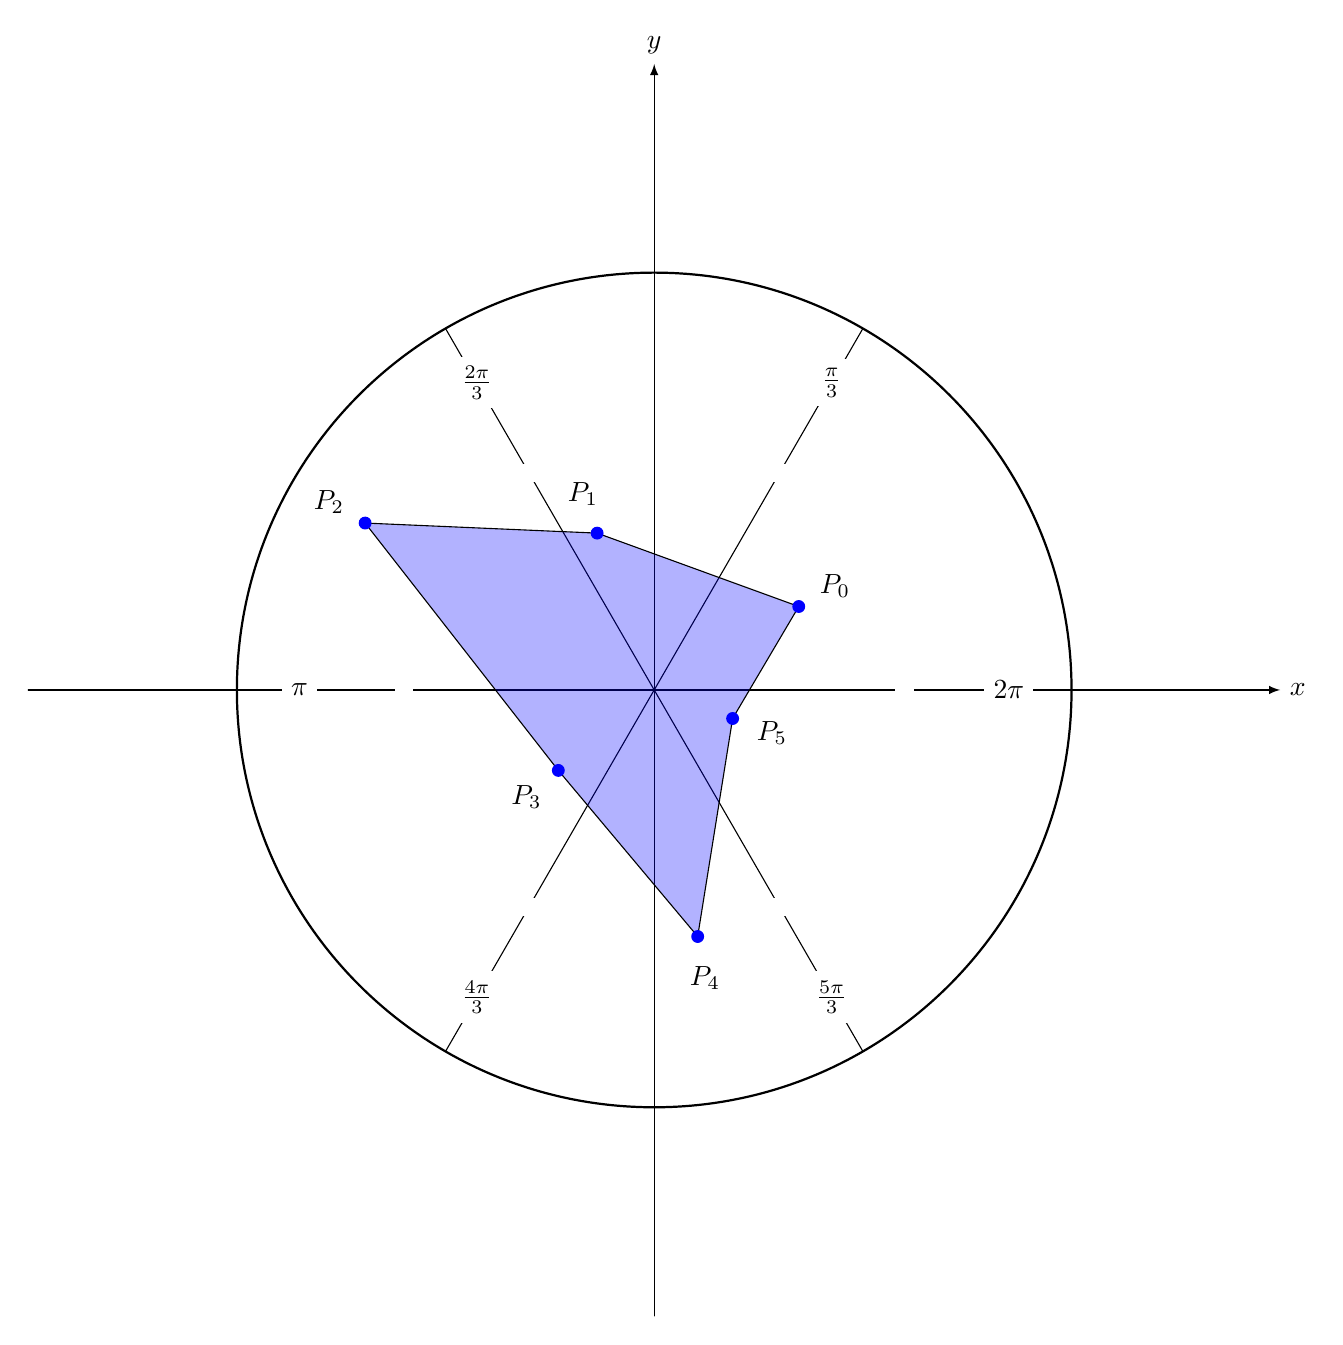
\begin{tikzpicture}[scale=5.3,cap=round,>=latex]

  % draw the coordinates
  \draw[->] (-1.5cm,0cm) -- (1.5cm,0cm) node[right,fill=white] {$x$};
  \draw[->] (0cm,-1.5cm) -- (0cm,1.5cm) node[above,fill=white] {$y$};

  % draw the unit circle
  \draw[thick] (0cm,0cm) circle(1cm);

  \foreach \x in {0,60,...,359} {
    % lines from center to point
    \draw[black] (0cm,0cm) -- (\x:1cm);
    % dots at each point
    %\filldraw[black] (\x:1cm) circle(0.4pt);
    % draw each angle in degrees
    \draw (\x:0.6cm) node[fill=white] {};
  }

  \coordinate (P0) at (30:0.4cm);
  \coordinate (P1) at (110:0.4cm);
  \coordinate (P2) at (150:0.8cm);
  \coordinate (P3) at (220:0.3cm);
  \coordinate (P4) at (280:0.6cm);
  \coordinate (P5) at (340:0.2cm);

  % Draw lines between body points
  \draw [fill=blue, fill opacity=0.3] (P0) -- (P1) -- (P2) -- (P3) -- (P4) -- (P5) -- cycle;

  % Draw body points
  \filldraw[blue] (P0) circle(0.4pt);
  \filldraw[blue] (P1) circle(0.4pt);
  \filldraw[blue] (P2) circle(0.4pt);
  \filldraw[blue] (P3) circle(0.4pt);
  \filldraw[blue] (P4) circle(0.4pt);
  \filldraw[blue] (P5) circle(0.4pt);

  % Draw body point labels
  \draw (30:0.5cm) node[fill=white] {\(P_{0}\)};
  \draw (110:0.5cm) node[fill=white] {\(P_{1}\)};
  \draw (150:0.9cm) node[fill=white] {\(P_{2}\)};
  \draw (220:0.4cm) node[fill=white] {\(P_{3}\)};
  \draw (280:0.7cm) node[fill=white] {\(P_{4}\)};
  \draw (340:0.3cm) node[fill=white] {\(P_{5}\)};

  % Draw each angle in radians
  \foreach \x/\xtext in {
    60/\frac{\pi}{3},
    120/\frac{2\pi}{3},
    180/\pi,
    240/\frac{4\pi}{3},
    300/\frac{5\pi}{3},
    360/2\pi} {
        \draw (\x:0.85cm) node[fill=white] {$\xtext$};
  }

  % draw the horizontal and vertical coordinates
  % the placement is better this way
  %\draw (-1.25cm,0cm) node[above=1pt] {$(-1,0)$}
  %     (1.25cm,0cm)  node[above=1pt] {$(1,0)$}
  %     (0cm,-1.25cm) node[fill=white] {$(0,-1)$}
  %     (0cm,1.25cm)  node[fill=white] {$(0,1)$};

\end{tikzpicture}
